\chapter{Introdu\c{c}\~{a}o}

A indústria de jogos eletrônicos é um dos segmentos de entretenimento mais rentáveis do mundo atualmente, superando, por exemplo, a indústria do cinema e da música \cite{newzoo1} \cite{ifpi1} \cite{mpaa1}. Conforme \cite{newzoo1}, o mercado de jogos eletrônicos alcançou mais de 99,5 bilhões de dólares em 2016. Um fator importante para esse sucesso é a possibilidade de jogar online e construir equipes com jogadores de todo o mundo.

Um segmento de jogo muito popular atualmente é o esporte eletrônico, mais conhecido como \textit{eSport} \cite{forbes1}. Conforme \cite{newzoo2}, o mercado de \textit{eSport} alcançou 493 milhões de doláres e uma audiência global de 191 milhões de entusiastas em 2016. O \textit{eSport} mais popular e rentável do mundo hoje é o League of Legends (LoL)  \cite{superdata1}, desenvolvido pela Riot Games, com cerca de 67 milhões de jogadores ativos e um pico diário de mais de 7,5 milhões de jogadores \textit{online} simultâneos \cite{riot1}.

LoL é um jogo de arena de batalha \textit{online} para vários jogadores (\textit{Multiplayer Online Battle Arena} - MOBA), um subgênero de jogos eletrônicos de estratégia em tempo real (\textit{Real-time Strategy} - RTS). Uma partida em um MOBA consiste em um cenário em que duas equipes lutam entre si, a fim de destruir a base do oponente como o principal objetivo, sem limite de tempo. Em geral, uma equipe tem cinco jogadores e cada um seleciona e controla um personagem com atributos e habilidades distintas. Além disso, as equipes também contam com a assistência de estruturas de defesa e unidades controladas por inteligência artificial para vencer a partida. Ao longo de uma partida, os personagens ganham ouro - que é usado para comprar itens para melhorar seus atributos e habilidades - e experiência de várias maneiras, como matar unidades ou personagens e destruir estruturas da equipe inimiga \cite{league1}.

A grande diversidade e dinamidade das ações dos personagens nas partidas \cite{drachen2014skill}, bem como seus desempenhos individuais (ou seja, ouro ganho, campeões derrotados, dano causado, cura recebida, etc.) tornam os MOBAs jogos muito competitivos. Em LoL, esta competitividade é ampliada devido à sua popularidade e torneios que fazem com que muitos jogadores se comportem como desportistas profissionais \cite{rioult2014mining}.

Dominar LoL é muito desafiador e requer um investimento substancial de tempo \cite{drachen2014skill}, principalmente para equipes inexperientes que não sabem inicialmente como elaborar ou melhorar sua estratégia. Nesse sentido, uma alternativa que poderia ajudar essas equipes é fornecer informações que levem a melhores decisões no jogo, como por exemplo, métricas de desempenho baseadas no comportamento de equipes bem-sucedidas. Isso levanta várias questões de pesquisa, como por exemplo:

\begin{enumerate}[label=(\roman*)]
  \item É possível identificar padrões úteis no comportamento de desempenho das equipes?
  \item É possível caracterizar perfis de equipes bem-sucedidas ou não usando esses padrões?
  \item É possível quantificar métricas de desempenho dos perfis de equipes?
\end{enumerate}

Até onde sabemos, ainda existe uma escassez de trabalhos acadêmicos que exploram esse assunto em \textit{eSports} \cite{drachen2014skill} \cite{ong2015player}, especialmente sobre comportamento de equipes de LoL.

Portanto, apresentamos e discutimos nesta dissertação os resultados de uma abordagem baseada em dados para identificar e caracterizar padrões de comportamento de equipes no contexto de LoL, o que nos leva a definir perfis de equipes bem-sucedidas e malsucedidas e suas métricas de desempenho. Primeiro, coletamos partidas do site de histórico de partidas de LoL. Em seguida, modelamos um conjunto de dados de equipes extraindo e resumindo fatores a partir de estatísticas sumarizadas de desempenho individual dos jogadores nas partidas. Depois, realizamos outras tarefas de engenharia de fatores, tais como limpeza de dados, remoção de fatores com baixa variância, detecção de \textit{outliers}, transformação de dados, normalização e análise de redundância. Para descobrir padrões de comportamento, aplicamos um método de aprendizado de máquina (K-means) no conjunto de dados de equipes para descobrir um número ótimo de grupos e, assim, agrupar equipes similares. Finalmente, caracterizamos cada grupo por meio de análise exploratória de dados e análise de relevância. Os resultados implicam que alguns grupos são mais propensos a ganhar do que outros e a influência dos fatores é distinta para cada um, o que nos permitiu definir perfis de equipe e métricas de desempenho.

\section{Objetivos}
\section{Contribuições}
\section{Estrutura da Dissertação}

\chapter{Fundamentação Teórica}
\section{MOBA}
\subsection{League of Legends}
\section{Mineração de Dados}
\subsection{Aprendizado supervisionado}
\subsection{Aprendizado não supervisionado}
\subsection{Seleção e extração de fatores}

\chapter{Trabalhos Relacionados}

Um conjunto de publicações tem investigado sobre MOBAs por meio de análise de dados e mineração de dados para realizar diversas tarefas.

Riolut et al. \cite{rioult2014mining} investigam como o comportamento dos jogadores em Dota 2, outro MOBA popular desenvolvido pela Valve Corporation, é relevante para prever o resultado das partidas a partir de dados posicionais dos jogadores nas partidas. Conley et al. \cite{conley2013does} e Kalyanaraman \cite{kalyanaraman2014win} apresentam, cada, um preditor de resultados de partidas e um recomendador de heróis com base em dados de composição de heróis (personagens) de equipes de Dota 2, onde cada observação corresponde a um vetor que codifica a presença ou não de um herói escolhido por um jogador na equipe. Kinkade e Lim \cite{kinkade2015dota} apresentam dois preditores de resultados de partidas de Dota 2: um preditor usa dados sumarizados do estado final das partidas e outro usa dados de composição de heróis. Ong et al. \cite{ong2015player} apresentam uma abordagem para agrupar diferentes comportamentos de desempenho individual dos jogadores e, assim, prever a equipe vencedora de uma partida com base na composição de comportamentos de jogadores das equipes. Johansson e Wikstr\"om \cite {johansson2015result} criam um modelo para prever a equipe vencedora de uma partida de Dota 2, usando dados parciais coletados à medida que uma partida avança. Schubert et al. \cite{schubert2016esports} apresentam uma técnica para segmentar dados de jogadores de Dota 2 nas partidas de maneira espacial e temporal onde cada segmento é referenciado como encontro de combate e, assim, possibilitar análises de desempenho e prever resultados de partidas com base nesses encontros.

Edge \cite{edge2013predicting} cria um modelo para prever quando os jogadores abandonarão uma partida de Dota 2 antes de terminar, modelando o estado motivacional dos jogadores na partida. Yang et al. \cite{yang2014identifying} modelam interações entre os jogadores em partidas de Dota 2 como uma sequência de grafos para identificar padrões de combate bem-sucedidos e, assim, prever resultados de combates durante a partida. Eggert et al. \cite{eggert2015classification} apresentam uma abordagem para classificar o papel de um jogador dentro de uma equipe de Dota 2 a partir de dados sumarizados de eventos de baixo nível na partida.

Kim et al. \cite{kim2015efficiently} propõem um método baseado em dados multimodais de jogadores de LoL durante uma partida (teclado e mouse, tela do jogo, expressão facial, volume e movimento do jogador) para detectar automaticamente as vezes em que esses jogadores exibem um comportamento atípico específico, como excitação, concentração, imersão e surpresa. Cavadenti et al. \cite{cavadenti2016did} propõem um método que ajude os jogadores da Dota 2 a melhorar suas habilidades descobrindo padrões estratégicos atípicos bem-sucedidos a partir de traços comportamentais históricos, ou seja, dado um modelo que codifica uma maneira esperada de se jogar (a norma), eles investigam padrões que se desviam da norma que pode explicar o resultado de uma partida.

Shim et al. \cite{shim2014decision} propõem um esquema de suporte à decisão de jogador automático com base em dados da antiga plataforma de denúncia do LoL (O Tribunal) para encontrar jogadores com mau comportamento (tóxico), como abusos e ataques maliciosos contra outros jogadores. Kwak e Blackburn \cite{kwak2014linguistic} realizam uma série de análises linguísticas para caracterizar o comportamento linguístico de jogadores tóxicos em League of Legends usando dados de contribuição colaborativa (\textit{crowdsourcing}) de jogadores acusados como tóxicos. Blackburn e Kwak \cite{blackburn2014stfu} exploram o uso do desempenho no jogo, relatórios de vítimas de comportamentos tóxicos e características linguísticas de mensagens de jogadores tóxicos em LoL para treinar classificadores para detectar a presença e gravidade de toxicidade. Shores et al. \cite{shores2014identification} examinam a natureza e os efeitos do comportamento tóxico em League of Legends para desenvolver uma métrica chamada índice de toxicidade e investigar os efeitos da interação de outros jogadores com jogadores tóxicos, incluindo taxa de retenção de jogadores.

Pobiedina et al. \cite{pobiedina2013ranking} analisam padrões de comportamento social de trabalho em equipe usando dados de comunidades virtuais de Dota 2. Park e Kim \cite{park2014social} analisam a rede social de jogadores de LoL para encontrar conhecimento relevante que ajude, por exemplo, a entender como os jogadores formam equipes. Drachen et al. \cite{drachen2014skill} apresentam um método para investigar como o comportamento das equipes em Dota 2 varia dependendo do nível de habilidade dos jogadores, analisando seus movimentos e a distância entre eles ao longo da partida. Claypool et al. \cite{claypool2015surrender} analisam dados quantitativos e qualitativos de partidas de LoL, como duração da partida e contentamento do jogador, para investigar se partidas criadas automaticamente (\textit{matchmaking}) são equilibradas ou não. Neidhardt et al. \cite{neidhardt2015team} investigam os impactos de três categorias de fatores de equipe (habilidades dos jogadores, relações de colaboração e parcerias com jogadores em equipes anteriores) em relação ao desempenho das equpes e duração das partidas de Dota 2. Leavitt et al. \cite{leavitt2016ping} analisam jogadores em partidas da League of Legends para investigar o impacto do sistema de comunicação não-verbal (\textit{ping}) no desempenho das equipes. Buchan e Taylor \cite{buchan2016qualitative} exploram o jogo em equipe analisando as experiências subjetivas dos participantes (tais como comunicação, papel, estado psicológico e nível de habilidade de jogo) ao jogar MOBAs e, assim, criar um modelo conceitual baseado em processos de grupo tradicionais (papéis de equipe, desenvolvimento de grupo e percepções e comportamento durante o estado de desvinculação). Kim et al. \cite{kim2017makes} examinam quais fatores individuais e de grupo estão associados à inteligência colaborativa em equipes de LoL e se ela é preditiva para o desempenho dessas equipes, com base em conjuntos de dados que compreendem métricas no jogo, resultados laboratoriais e questionários de equipes.

Embora estes estudos desempenhem um papel essencial na literatura, nenhum deles se propôs a modelar perfis de equipe em LoL com base no comportamento de desempenho das equipes nas partidas, bem como, fornecer métricas de desempenho bem-sucedidas de equipes que possa apoiar a tomada de decisão.

\chapter{Preparação dos Dados}
Para preparar o conjunto de dados de equipes, foram realizadas as seguintes tarefas: coleta de dados, limpeza de dados; remoção de fatores com baixa variância; detecção de \textit{outliers}; transformação de dados; normalização de dados; e análise de redundância de fatores.

\subsection{Coleta de Dados}
LoL developer, Riot Games, provides a web-based Application Public Interface (API) to access match histories in JSON format \cite{riot1}. A match history contains data such as game mode\footnote{The classic mode is the most chosen by the players and a match must have 10 participants dueling each other for two different teams.}, queue type\footnote{A player needs to enter the queuing system to participate in a match, and there are several types of queues.}, match duration, winner/loser team and identification number. It also contains data from each player participating in the match as character choice and summarized performance statistics. These statistics indicate, for example, total damage dealt/taken, gold earned/spent, damage dealt/spent and healing received. Table ~\ref{tab:features-desc} shows the descriptions of the statistics. We randomly collected over 110,000 match histories from February to December 2016 (10,000 for each month), considering the following filters: \textit{Region} Brazil; \textit{Season} 2016; \textit{Match mode} Classic; \textit{Queue type} Ranked solo; \textit{Total players in each team} 5; \textit{Match version} 6.x.x.

Then we extracted the features to model our teams' dataset from collected matches. Let $M=\{m_1,...,m_{110000}\}$ be a set of matches, $T=\{t_1, ..., t_n | n=110000 * 2\}$ a set of teams, $P=\{p_1, ..., p_{|P|}\}$ a dimensional $d=38$ set of players' total performance statistics. A match consists of two distinct teams $m=\{t_a,t_b\}$ and a team consists of 5 distinct players $t=\{p_k |  p_k \in P^t; P^t \supset P; 1 \geq k \leq 5\}$. We selected the players' total performance statistics in matches and summarized each one $P_j \in P$ by team in order to form our teams' dataset features $X_j \in X_{220000, 38}$ as follows: $X_j= \sum_{t \in T}{} P_{j}^{t}$.

Finally, to guarantee data atomicity, we subtracted \textit{physicalDamageDealt} from \textit{physicalDamageDealtToChampions} to compute \textit{physicalDamageDealtToMonsters} and \textit{magicDamageDealt} from \textit{magicDamageDealtToChampions} to compute \textit{magicDamageDealtToMonsters}. We also removed compounded features to avoid redundancy, for example, \textit{totalDamageDealt} which is the sum of \textit{physicalDamageDealt} and \textit{magicDamageDealt}. Table ~\ref{tab:features-desc} also shows the compounded features marked with (*) we removed.

\begin{table}
  \tiny
  \caption{Descriptions of players' performance statistics.}
  \label{tab:features-desc}
  \begin{tabular}{p{0.13\textwidth}p{0.29\textwidth}}
    \toprule
    Feature & Description \\
    \midrule
assists & Number of assists\\
deaths & Number of deaths\\
doubleKills & Number of double kills\\
goldEarned & Gold earned\\
goldSpent & Gold spent\\
inhibitorKills & Number of inhibitor kills\\
killingSprees & Number of killing sprees\\
kills & Number of kills\\
largestCriticalStrike & Largest critical strike\\
largestKillingSpree & Largest killing spree\\
largestMultiKill & Largest multi kill\\
magicDamageDealt* & magicDamageDealtToChampions +  magicDamageDealtToMonsters\\
magicDamageDealtToChampions & Magical damage dealt to champions\\
magicDamageTaken & Magic damage taken\\
minionsKilled & Minions killed\\
 neutralMinionsKilled* & neutralMinionsKilledEnemyJungle + neutralMinionsKilledTeamJungle\\
neutralMinionsKilledEnemyJungle & Neutral jungle minions killed in the enemy team' jungle\\
neutralMinionsKilledTeamJungle & Neutral jungle minions killed in your team's jungle\\
pentaKills & Number of penta kills\\
physicalDamageDealt* & physicalDamageDealtToChampions + physicalDamageDealtToMonsters\\
physicalDamageDealtToChampions & Physical damage dealt to champions\\
physicalDamageTaken & Physical damage taken\\
quadraKills & Number of quadra kills\\
sightWardsBoughtInGame & Sight wards purchased\\
totalHeal & Total heal amount\\
totalTimeCrowdControlDealt & Total dealt crowd control time\\
totalUnitsHealed & Total units healed\\
towerKills & Number of towers the team destroyed\\
tripleKills & Number of triple kills\\
totalDamageDealt* & physicalDamageDealt + magicDamageDealt \\
totalDamageDealtToChampions* & physicalDamageDealtToChampions + magicDamageDealtToChampions \\
 trueDamageDealt* & trueDamageDealtToChampions + trueDamageDealtToMonsters\\
trueDamageDealtToChampions & True damage dealt to champions\\
trueDamageTaken & True damage taken\\
visionWardsBoughtInGame & Vision wards purchased\\
wardsKilled & Number of wards killed\\
wardsPlaced & Number of wards placed\\
  \bottomrule
\end{tabular}
\end{table}

\subsection{Análise Descritiva}
\subsection{Extração de Fatores}
\subsection{Limpeza de Dados}
\subsection{Remoção de Fatores com Baixa Variância}
\subsection{Detecção de Outliers}
\subsection{Transformação de Dados}
\subsection{Normalização}
\subsection{Análise de Redundância}

\section{Se\c{c}\~{a}o 1 do Capítulo 1}
\subsection{Subseção}
\subsubsection{Subsubseção}

A Figura \ref{fig:sistemaProposto}. A Tabela \ref{tab:tabelaTeste}. A Equacao (\ref{eq1}). O trabalho de fulano ~\cite{ref1}. O Codigo Fonte \ref{cod1}.

\begin{figure}[htbp]	
\begin{center}
		\fbox{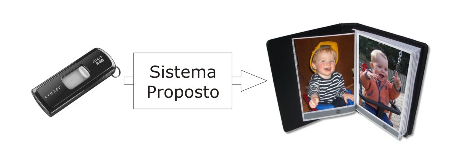
\includegraphics[scale=1]{sistemaProposto.eps}}
	\end{center}
	\caption{Sistema proposto}
	\label{fig:sistemaProposto}
\end{figure}

\begin{table}[htpb]
\begin{center}
\begin{tabular}{|c|c|c|}
\hline
coluna 1 & coluna 2 & coluna 3 \\
\hline
valor 1,1 & valor 1,2 & valor 1,3 \\
valor 2,1 & valor 2,2 & valor 2,3 \\
\hline
\end{tabular}
\end{center}
\caption{Primeira tabela.}
\label{tab:tabelaTeste}
\end{table}

\begin{equation}
E = m \times c^2
\label{eq1}
\end{equation}

\begin{lstlisting}[caption={Loop simples},label=cod1,numbers=none]
for(int x=1; x<10; x++){
  cout << x << "\n";
}
\end{lstlisting}

\section{Se\c{c}\~{a}o 2 do Capítulo 1}  
\subsection{Subseção}
\subsubsection{Subsubseção}

